%% Be sure to check spelling!

%% Put your name and the proper due date in place!

\documentclass{article}
\usepackage{amsmath}    % loads AMS-Math package
\usepackage{graphicx}   % bring in graphics
\usepackage{listings}   % allows lstlisting environment
\usepackage[letterpaper, margin=0.5in]{geometry}  % set paper size/margins
\usepackage{EGR103style}  % colorful file imports
\begin{document}
\begin{center}
\rule{6.5in}{0.5mm}\\~\\
\textbf{\large EGR 103L -- Fall 2021}\\~\\
\textbf{\huge \LaTeX~Assignment}\\~\\
*** NAME (NetID) ***\\
*** Lab Section N, DAY TIMES ***\\
*** DATE DUE ***\\~\\
{\small I understand and have adhered to all the tenets of the Duke Community Standard in completing every part of this assignment.  I understand that a violation of any part of the Standard on any part of this assignment can result in failure of this assignment, failure of this course, and/or suspension from Duke University.} 
\rule{6.5in}{0.5mm}\\
\end{center}
\tableofcontents
\listoffigures
\pagebreak

\section{Equations} %%% You will add your equations here
\begin{itemize}
\item General second-order system equation\cite[p.~221]{Rizzoni}:
% unnumbered and aligned equation
\item The Secant Formula for finding maximum stress 
in a column\cite[p.~681]{Hibbeler}:
% unnumbered and aligned equation
\item Characteristic determinant for a 2x2 system of 
differential equations\cite[p.~152]{Kreyszig}:
% aligned numbered equations...except no numbers on first parts
\item Definition of the Lyapunov exponent\cite[p.~56]{Ott}:
% aligned numbered equations
\end{itemize}

\section{Tables using \texttt{tabular} and \texttt{array}}
\subsection{Using \texttt{tabular}} %%% You will add the tabular here
Converting ammonia into nitric acid - the Ostwald Process\cite{Ostwald}:
% centered tabular here
\subsection{Using \texttt{array}} %%% You will add the array here
% stretched array here
\pagebreak

\section{Comments} %%% You will add your comments here
Things I learned in this assignment:
% itemized list here

\pagebreak
\appendix
\section{Codes}
%%% Everything in this section is done; make sure you 
%%% understand how it works in general
\lstset{style=python103, language=python} 
% above changes all listings to python style from EGR103S19
\subsection{Listing of full sample header for original code}
\lstinputlisting{Header1f.py}
\subsection{Listing of short sample header for original code}
\lstinputlisting{Header1s.py}
\subsection{Listing of full sample header for modified code}
\lstinputlisting{Header2f.py}
\subsection{Listing of short sample header for modified code}
\lstinputlisting{Header2s.py}
\pagebreak
\subsection{Listing code for sample graph on following page}
\lstinputlisting{MakeSample.py}

\pagebreak
\section{Figures \label{FigureList}}
%%% Everything in this section is done; make sure you 
%%% understand how it works in general

\begin{figure}[htb]
\begin{center}
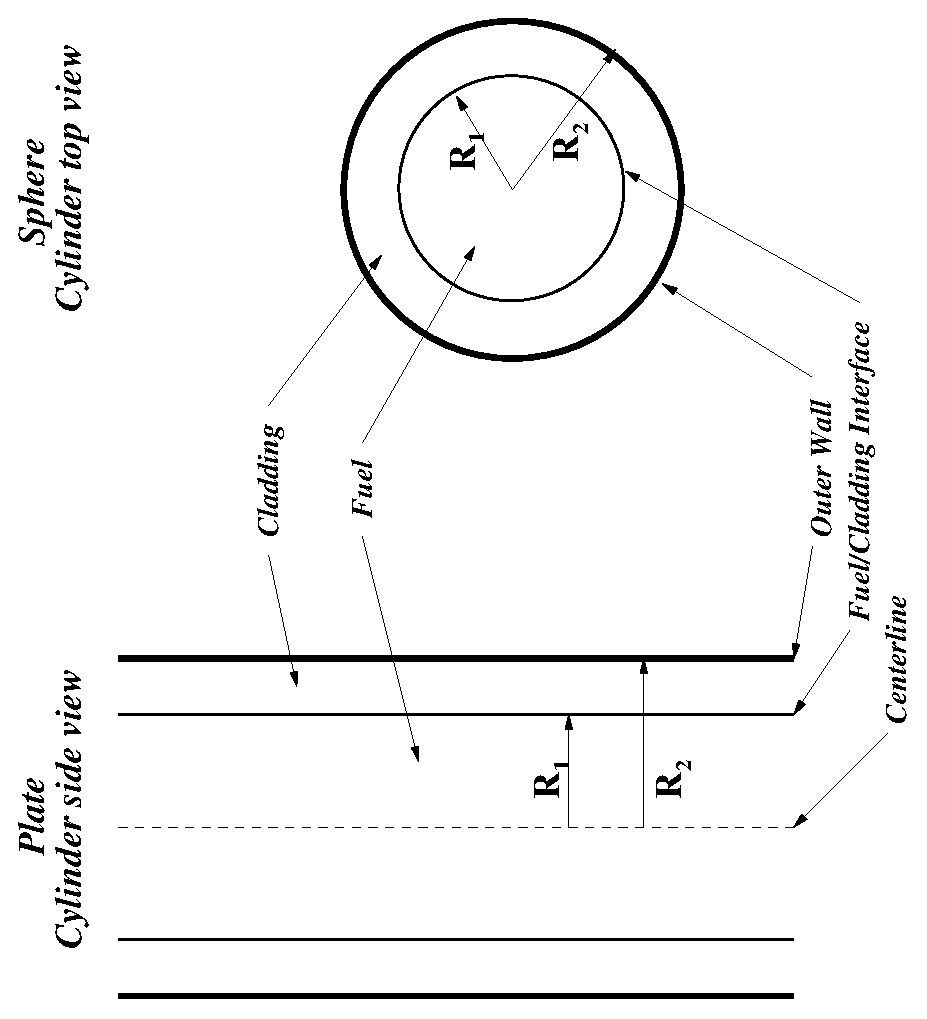
\includegraphics[angle=-90, width=4in]{drawing.eps}
\caption{Drawing from ME 431L test.}
\end{center}
\end{figure}

\begin{figure}[!h]
\begin{center}
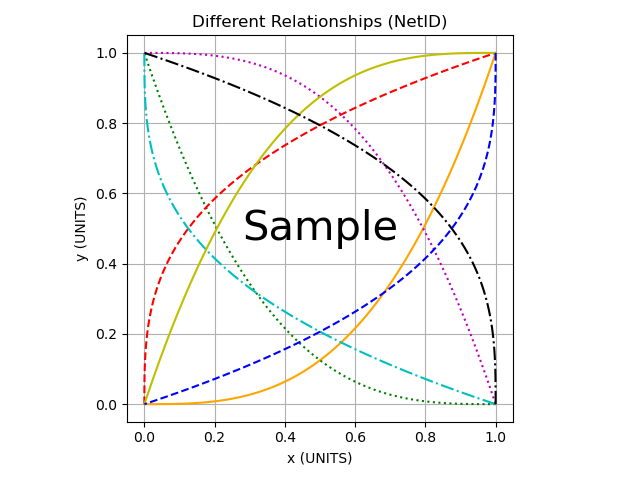
\includegraphics[width=5in]{SamplePyplot.png}
\caption{Sample figure.}
\end{center}
\end{figure}
\pagebreak

%%% Everything in this section is done; make sure you 
%%% understand how it works in general
%%% Note that line returns are optional
\addcontentsline{toc}{section}{References}
\begin{thebibliography}{9}
\bibitem{Rizzoni}
  Rizzoni, Georgio,
  {\it Principles and Applications of Electrical Engineering}.
  McGraw-Hill, New York,
  5th Edition,
  2007.
\bibitem{Hibbeler}
Hibbeler, R. C.,
{\it Mechanics of Materials}.
Pearson Prentice Hall, Upper Saddle River, NJ, 8th Edition, 2011.
\bibitem{Kreyszig}
Kreyszig, Erwin,
{\it Advanced Engineering Mathematics}.
John Wiley \& Sons, New York, 8th Edition, 1999.
\bibitem{Ott}
Ott, Edward,
{\it Chaos in Dynamical Systems}.
Cambridge University Press, Cambridge, UK, 1st Edition, 1993.
\bibitem{Ostwald}
Wikipedia, 
{\it Ostwald process} (http://en.wikipedia.org/wiki/Ostwald$\_$process).
Online; accessed 19-Aug-2012.
\end{thebibliography}

\end{document}
